\documentclass[10.5pt,compsoc]{TsT}
\usepackage{graphicx}
\usepackage{footmisc}
\usepackage{subfigure}
\usepackage{url}
\usepackage{multirow}
\usepackage[noadjust]{cite}
\usepackage{amsmath,amsthm}
\usepackage{amssymb,amsfonts}
\usepackage{booktabs}
\usepackage{color}
\usepackage{ccaption}
\usepackage{booktabs}
\usepackage{float}
\usepackage{fancyhdr}
\usepackage{caption}
\usepackage{xcolor,stfloats}
\usepackage{comment}
\setcounter{page}{1}
\graphicspath{{figures/}}
\usepackage{cuted}  %flushend,
\usepackage{captionhack}
\usepackage{epstopdf}
%\usepackage[lite,subscriptcorrection,slantedGreek,nofontinfo]{mtpro2}

%===============================%
\headevenname{\zihao{-5}{\textbf{\emph{Tsinghua Science and Technology, June}}} 2013, 18(3): 000-000}%
\headoddname{{\sf Wang Zhenyang et al.:}\quad {\textbf{\emph{Attention to Difficult Instances: A Cascade Coarse to Fine Network Architecture for Semantic Segmentation}}}}%
%footnote use of *
\renewcommand{\thefootnote}{\fnsymbol{footnote}}
\newcommand{\upcite}[1]{\superscript{\textsuperscript{\cite{#1}}}}
\setcounter{footnote}{0}
\renewcommand\footnotelayout{\normalsize}

\newtheoremstyle{mystyle}{0pt}{0pt}{\normalfont}{1em}{\bf}{}{1em}{}
\theoremstyle{mystyle}
\renewcommand\figurename{Fig.~}
\renewcommand{\thesubfigure}{(\alph{subfigure})}
\newcommand{\upcite}[1]{\textsuperscript{\cite{#1}}}
\renewcommand{\labelenumi}{(\arabic{enumi})}
\newcommand{\tabincell}[2]{\begin{tabular}{@{}#1@{}}#2\end{tabular}}
\newcommand{\abc}{\color{white}\vrule width 2pt}


\newtheorem{assumption}{\textbf{Assumption}}
\newtheorem{definition}{\textbf{Definition}}
\newtheorem{lemma}{\textbf{Lemma}}
\newtheorem{theorem}{\textbf{Theorem}}
\newtheorem{proposition}{\textbf{Proposition}}
\newtheorem{corollary}{\textbf{Corollary}}






%\newcommand{\TODO}[1]{\textbf{TODO: #1}}

\addtolength{\abovecaptionskip}{-2mm}
\addtolength{\belowcaptionskip}{-2mm}

%%% aanpassing van cite aan journal style
\makeatletter
%\def\@cite#1#2{\textsuperscript{[{#1\if@tempswa, #2\fi}]}}
\renewcommand{\@biblabel}[1]{[#1]\hfill}
\makeatother

\begin{document}

\thispagestyle{empty}



\hyphenpenalty=50000

\makeatletter
\newcommand\mysmall{\@setfontsize\mysmall{7}{9.5}}

%%%%%%%%%%%%%%%%%%%%%%%
\newenvironment{tablehere}
  {\def\@captype{table}}
  {}
\newenvironment{figurehere}
  {\def\@captype{figure}}
  {}
%%%%%%%%%%%%%%%%%%%%%%%
%%%%%%%%%%%%%%%%%%%%%%%%%%%%%%%%

\thispagestyle{plain}%
\thispagestyle{empty}%

\let\temp\footnote
\renewcommand \footnote[1]{\temp{\zihao{-5}#1}}
{}
\vspace*{-40pt}

%{\hbox
\noindent{\zihao{5-}\textbf{\scalebox{0.89}[1.0]{\makebox[5.6cm][s]{%
TSINGHUA SCIENCE AND TECHNOLOGY}}}}

\vskip .2mm
{\zihao{5-}
\textbf{
\hspace{-5mm}
\scalebox{1}[1.0]{\makebox[5.6cm][s]{%
I\hspace{0.70pt}S\hspace{0.70pt}S\hspace{0.70pt}N\hspace{0.70pt}{\color{white}%
l\hspace{0.70pt}l\hspace{0.70pt}}1\hspace{0.70pt}0\hspace{0.70pt}0\hspace{0.70pt%
}7\hspace{0.70pt}-\hspace{0.70pt}0\hspace{0.70pt}2\hspace{0.70pt}1\hspace{0.70pt%
}4\hspace{0.70pt}{\color{white}l\hspace{0.70pt}l\hspace{0.70pt}}0\hspace{0.70pt}%
?\hspace{0.70pt}/\hspace{0.70pt}?\hspace{0.70pt}?\hspace{0.70pt}{\color{white}%
l\hspace{0.70pt}l\hspace{0.70pt}}p\hspace{0.70pt}p\hspace{0.70pt}?\hspace{0.70pt}?\hspace{0.70pt}?%
-\hspace{ 0.70pt}?\hspace{0.70pt}?\hspace{0.70pt}?}}}

\vskip .2mm\noindent
{\zihao{5-}\textbf{\scalebox{1}[1.0]{\makebox[5.6cm][s]{%
V\hspace{0.8pt}o\hspace{0.8pt}l\hspace{0.8pt}u\hspace{0.8pt}m\hspace{0.8pt}%
e\hspace{0.6em}1\hspace{0.8pt}8,\hspace{0.6em}N\hspace{0.8pt}u\hspace{0.8pt}%
m\hspace{0.8pt}b\hspace{0.8pt}e\hspace{0.8pt}r\hspace{0.6em}3,\hspace{0.6em}%
J\hspace{0.8pt}u\hspace{0.8pt}n\hspace{0.8pt}e%
\hspace{0.6em}2\hspace{0.8pt}0\hspace{0.8pt}1\hspace{0.8pt}3}}}}


\begin{strip}
{\center \vskip 3mm
{\zihao{3}\textbf{
Attention to Difficult Pixels: A Cascade Coarse to Fine Network Architecture for Semantic Segmentation
}}
\vskip 9mm}

{\center {\sf \zihao{5}
Wang Zhenyang, Deng Zhidong$^*$, and Wang Shiyao
}
\vskip 5mm}
%{\center \zihao{-5}{\textbf{
%1.~School of Computer Science, China University of Geosciences, Wuhan 430074, China;  \\
%2.~Shandong Provincial Key Laboratory of Computer Network, Jinan 250014, China; \\
%3.~School of Electronic Engineering Naval University of Engineering, Wuhan 430033, China\\
%}}}
%
%\vskip 5mm

\centering{
\begin{tabular}{p{160mm}}

{\zihao{-5}
\linespread{1.6667} %
\noindent
\bf{Abstract:} {\sf
Scene labeling, based on semantic segmentation, is a fundamental topic in computer vision. The goal is to assign each pixel in the image a category label. Recently, convolutional neural networks have attracted increasing attention on semantic segmentation due to the capabilities of extracting hierarchical features. Since it is required to make dense predictions for each pixel, a simple network is hardly to obtain considerable performances on different scenes. In this paper, we propose a cascade coarse to fine network architecture, which aims to pay more attention to the difficult pixels. The network has three branches. The first branch is responsible for handling easier regions by producing coarse predictions. And the second branch learns to distinguish the relatively difficult pixels from the entire images. Subsequently, a few hard regions will be fed to the last branch in order to make further predictions which is help to improve the final performance. All above branches focus on their own objectives and collaboratively learn to predict from coarse to fine inference. In order to evaluate predicting performance of the proposed network, we conduct experiments on two public datasets including Sift Flow and Stanford Background Dataset. We show that the three branches can be trained in an end-to-end manner and the experimental results show that compared to all existing models, our HMNet consistently yields the best performance, with accuracy of 91.6\% and 89.7\%, respectively.
}
\vskip 4mm
\noindent
{\bf Key words:} {\sf 
semantic segmentation; online hard example mining; convolutional neural network
}}

\end{tabular}
}
\vskip 6mm

\vskip -3mm
\zihao{6}\end{strip}


\thispagestyle{plain}%
\thispagestyle{empty}%
\makeatother
\pagestyle{tstheadings}

\begin{figure}[b]
\vskip -6mm
\begin{tabular}{p{44mm}}
\toprule\\
\end{tabular}
\vskip -4.5mm
\noindent
\setlength{\tabcolsep}{1pt}
\begin{tabular}{p{1.5mm}p{79.5mm}}
$\bullet$& Wang Zhenyang, Deng Zhidong, Wang Shiyao are with the Department of Computer Science, Tsinghua University, Beijing 100084, China. E-mail: crazycry2010@gmail.com, michael@tsinghua.edu.cn, sy-wang14@mails.tsinghua.edu.cn \\
$\sf{*}$&
To whom correspondence should be addressed. \\
          &          Manuscript received: 2017-09-20; revised: year-month-day; accepted: year-month-day

\end{tabular}
\end{figure}\zihao{5}



%\vspace{3.5mm}
\section{Introduction}
\label{s:introduction}
\noindent

Semantic segmentation has a strong application requirement in the field of environment perception and autonomous self driving car. The goal of semantic segmentation is to identify and assign each pixel in the image a category label which requires a complete understanding of the semantic information of the entire image. In recent years, deep learning has made breakthroughs in image classification\upcite{1,2,3}, speech recognition\upcite{4}, object detection\upcite{5} and so on. For the task of image semantic segmentation, there are also many methods based on deep learning methods. Early research attempts to apply the convolution neural network designed for image recognition directly to semantic segmentation. Although good segmentation results are obtained, the prediction results are rough and the edges of objects  can not be separated correctly. This is mainly cased by the losing of location information. Consequently, a fully convolutional neural network is proposed by to overcome this disadvantage that becomes the most popular segmentation framework for semantic segmentation task.

Besides, in order to solve the problem of edge blur, conditional random field, Markov random field, Gaussian conditional random field, and other variations are proposed. However, with the development of CNN modules, especially the batch normalization\upsite{6} and ResNet\upcite{7}, an end-to-end training procedure can achieve the same or even a better segmentation results.

In addition, the unbalance of the easy and difficulty pixels can also wreck the convergence of the network. Aiming to  deal with the unbalanced distribution, we propose a novel semantic segmentation network framework based on the hard negative example mining.

In fact, hard sample mining is not a new concept. As early as 1994, Sung and Poggio proposed bootstrapping method in their face detection algorithm. The main purpose is to enhance the algorithm's capacity by changing the distribution of difficult samples. Inspired by the similar ideas, a cascade coarse to fine network architecture(CCFNet) is proposed. CCFNet is composed by three branches which share a same feature extraction network. The first branch is a coarse segmentation network which is able to handle the easy and confident regions. The second branch is an attention network used to predict the probability of being a hard example for each pixel. For these difficult pixels, the third segmentation branch is proposed to refine the final results. The proposed CCFNet uses a multi-branch network structure, integrating the prediction from two different branches with an attention module to obtain the final segmentation results.

In conclusion, we propose a cascade coarse to fine network architecture for semantic segmentation. Compared with the traditional semantic segmentation networks, CCFNet has the following characteristics: 


\begin{figure}
\centering
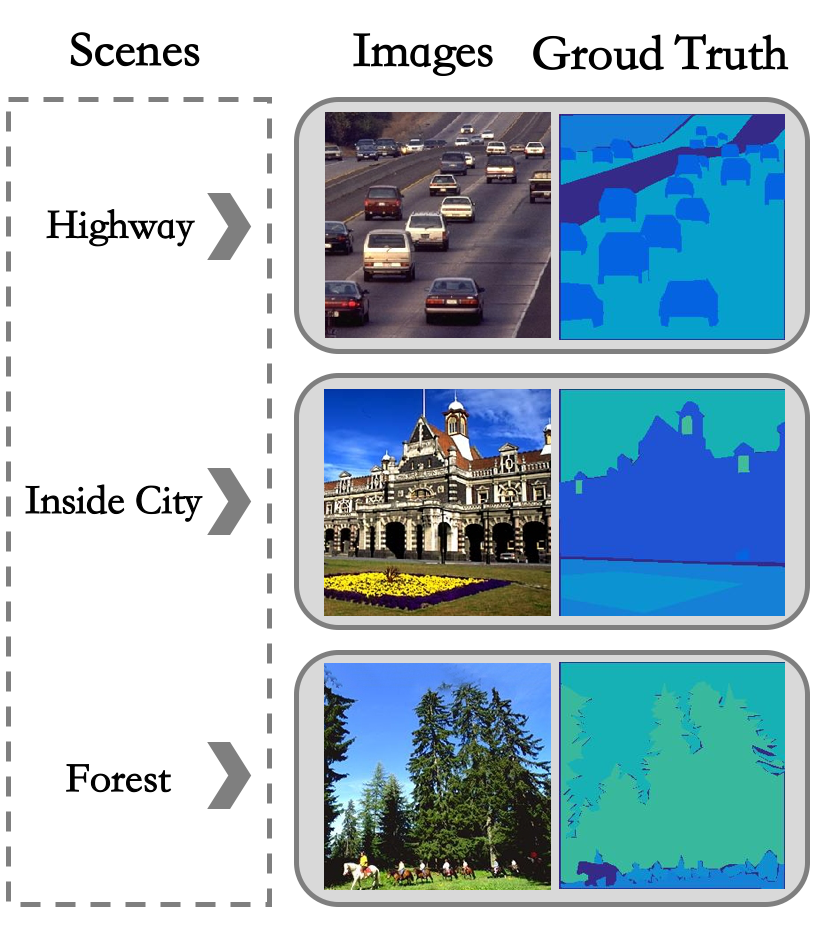
\includegraphics[width=0.95\columnwidth]{fig1.png}
\caption{Examples of semantic segmentation.}
\label{fig:example}
\end{figure} 


\noindent
  $\bullet$ A cascade segmentation network architecture to refine the final segmentation results.
  
\noindent
  $\bullet$ Incorporate the idea of hard mining into an attention module.
  
\noindent
  $\bullet$ Validate CCFNet on both Sift Flow Dataset\upcite{8} and Stanford Background Dataset\upcite{9}.


\section{Related Works}
\label{s:Related}
\noindent
Semantic segmentation aims to relate one semantic class (road, water, sea etc.) to each pixel of the input image. Both the global and local features have great impacts on the final performance of this task. Consequently, in terms of feature representations, the mainstream approaches can be divided into traditional hand-craft features and deep features based on deep neural networks. 

In recent years, traditional methods have obtained several solutions on image segmentation. Considering the context information, several methods rely on MRF, CRF or other types of graphical models to ensure consistency of labeling\upcite{10,11,12}. Besides, most methods employ pre-segmentation in order to produce super-pixels or segmented candidates, and extract features from these individual segments along with the combinations of adjacent segments.

Meanwhile, the neural networks, particularly the convolutional neural networks that yield hierarchies of features have achieved great progress in  this pixel-level prediction tasks. [13] is the first work that use CNNs for this semantic segmentation. They propose a multi-scale convolution neural network, which extracts the feature representations from different scales of local regions. The experimental results show that the network has capacities of learning texture, shape and domain information implicitly, and achieves better performance than traditional hand-craft features. In addition, the network is also able to generalized to the RGB-D images\upcite{14}. To ensure a good visual coherence and a high class accuracy, [15] propose a method to capture long range (pixel) label dependencies in images. They use a recurrent architecture for convolutional neural networks to capture a long range label dependency while keeping a tight control over the capacity. The procedure is based on supervised deep learning strategies. [16-18] train the parametric CNNs by sampling image patches, which speeds up the training time dramatically. However, they find that patch-based CNNs suffer from local ambiguity problems. [16] estimate the global potential in a non-parametric framework and propose a large margin based CNN metric for better global potential estimation. [17,18] introduce quaddirectional 2D Recurrent Neural Networks to model the long range dependencies among pixels which is able to embed the global image context into the compact local representation and significantly enhance their discriminative power.

At the same time, the researchers attempt to use the pre-trained convolution neural networks for semantic segmentation. [19] obtain the local and proximal features by using the ConvNet while distant and global features are produced from Alex-net\upcite{20}. These above features are further aggregated to predict the categories. Diff from these methods, [21] present a fully convolutional network which is able to take input of arbitrary size and produce correspondingly-sized output with efficient inference and learning. They use the CNNs trained on ImageNet as a feature extractor and transfer their learned representations by fine-tuning on the task-specific datasets. [22] propose deep networks by combining the responses at the final DCNN layer with a fully connected Conditional Random Field (CRF). The fully connected pairwise CRF has an ability to capture fine edge details which boosts the final performance. In [23], it presents that the main problem of the current FCN-based models is lack of the use of global context to help to make decision. They exploit the capability of global context information by different-region-based context aggregation through a pyramid pooling module together with the proposed pyramid scene parsing network (PSPNet).

\begin{figure*}[t]
\centering
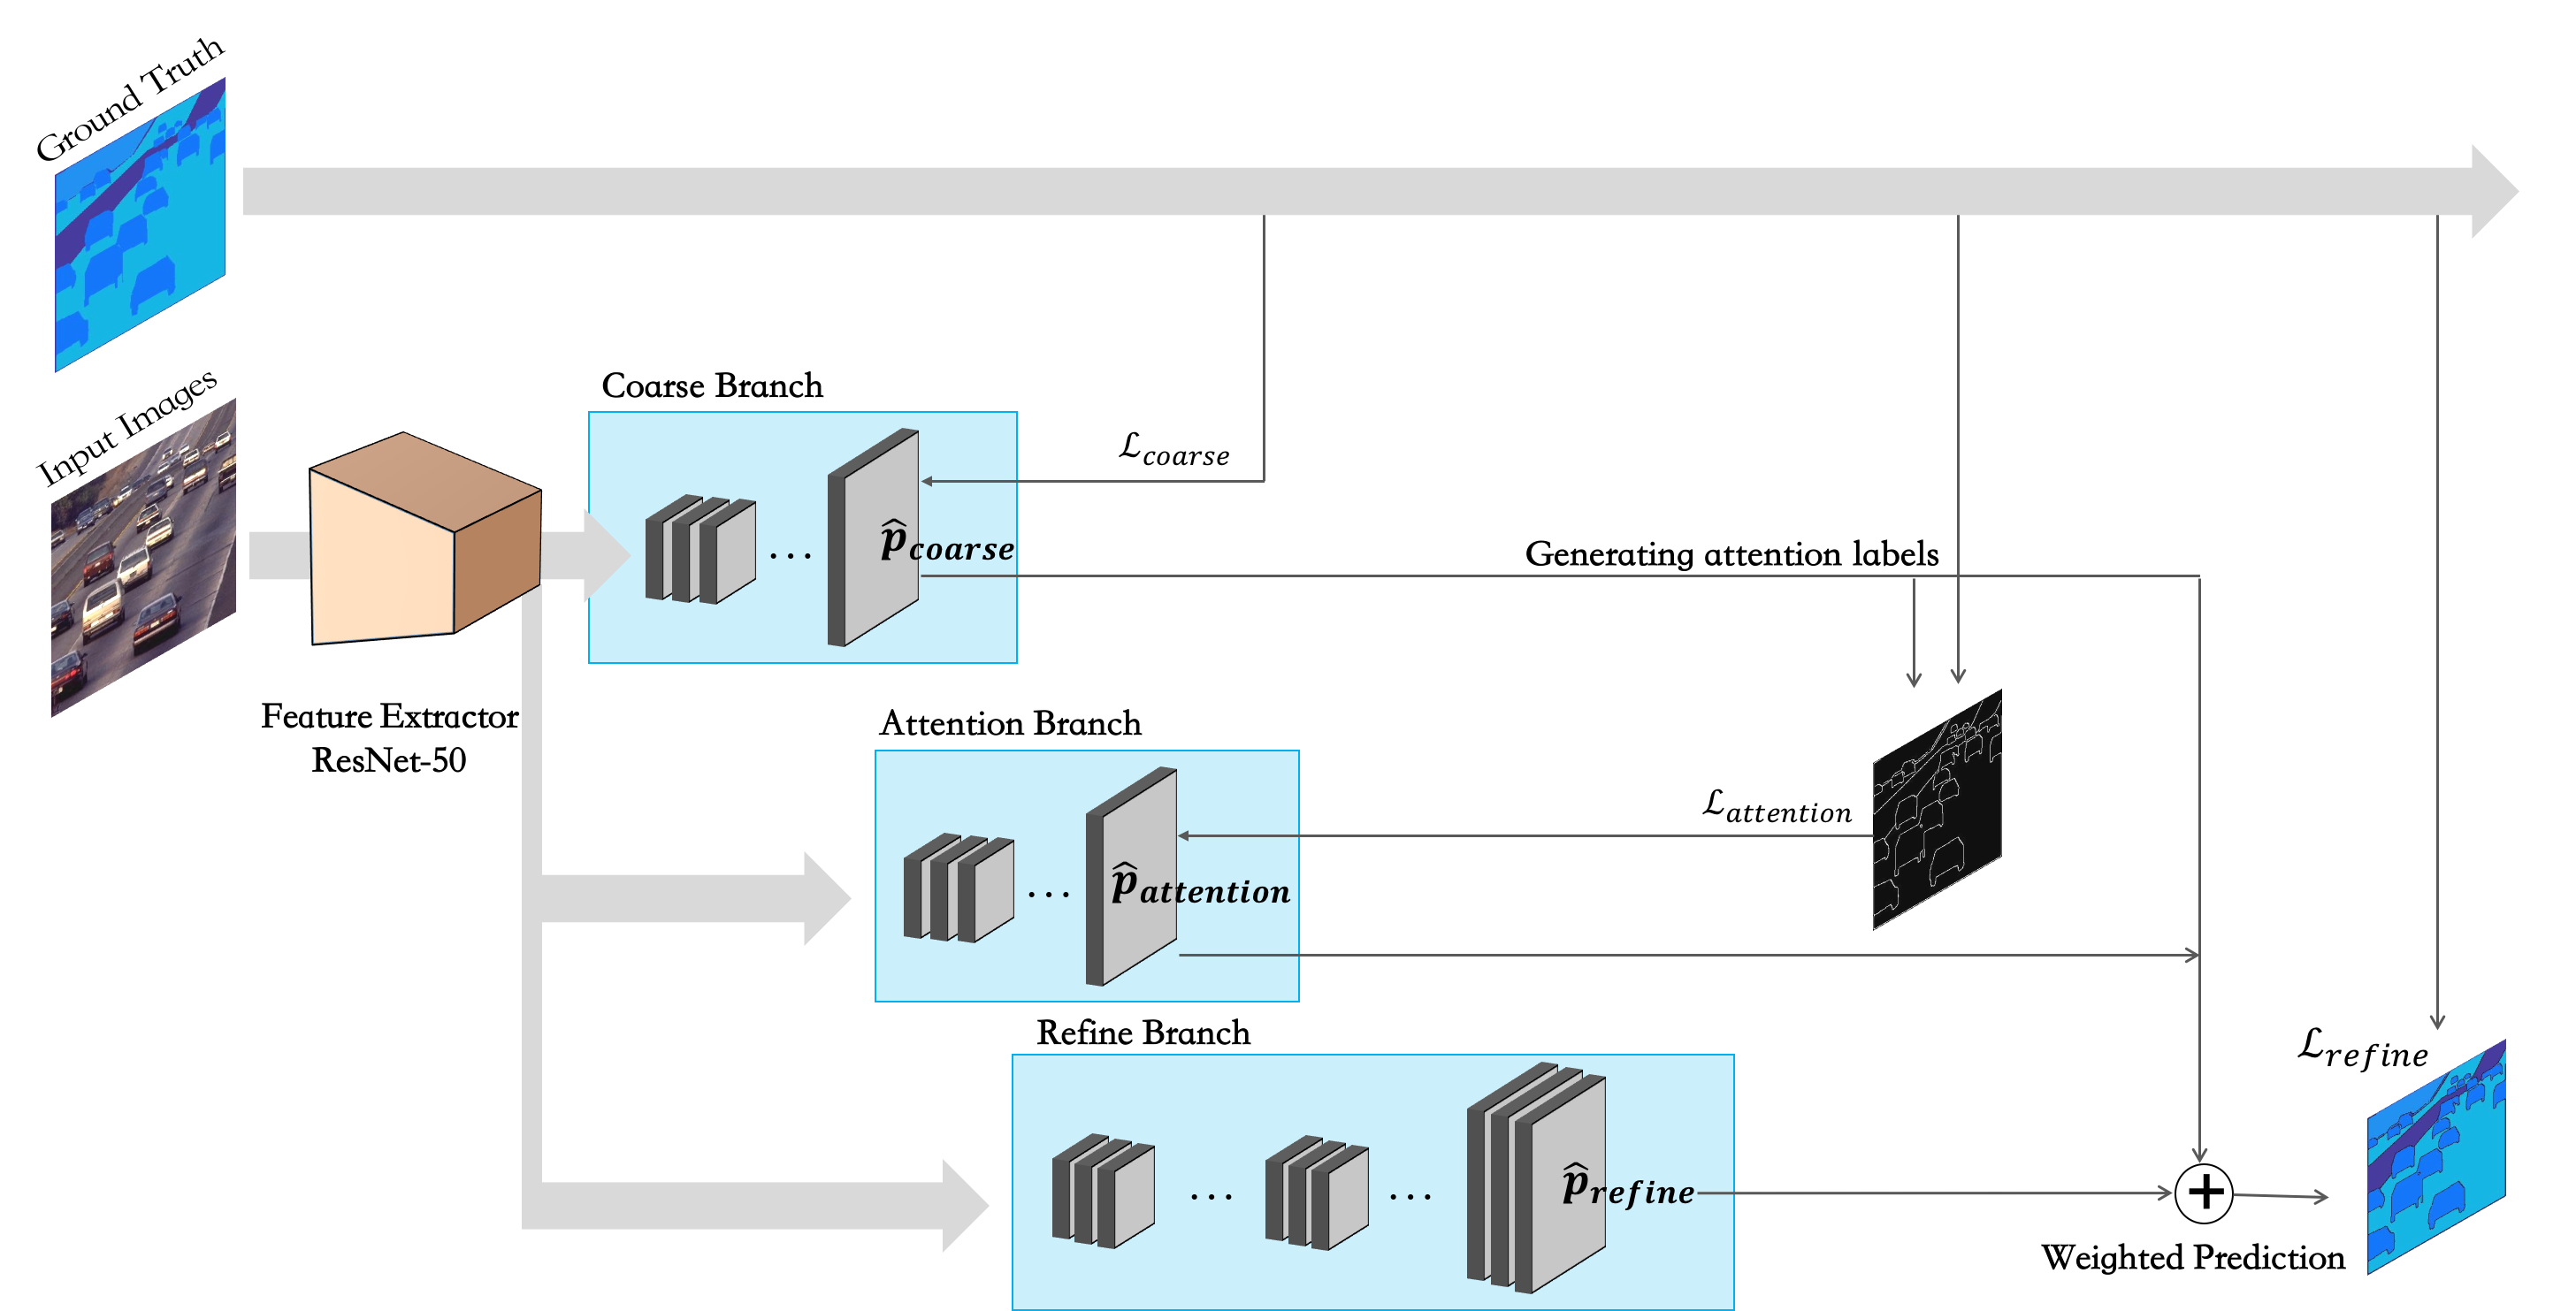
\includegraphics[width=1.9\columnwidth]{fig2.png}
\caption{A Cascade Coarse to Fine Network Architecture for Semantic Segmentation.}
\label{fig:arch}
\end{figure*} 

\section{Method}
\label{s:Method}
\noindent


Inspired by online hard example mining(OHEM) algorithm, we propose a cascade coarse to fine network architecture CCFNet. 
Section~\ref{s:arch} illustrates how to turn a ImageNet pre-trained model to a cascade coarse to fine semantic segmentation network CCFNet.
Taking the characteristics of semantic segmentation task into consideration, section~\ref{s:hard} introduces a hard instance mining method to learn the attention about the difficulty of each instance.
Section~\ref{s:hard} detailes the training and testing process of CCFNet. 
%The idea behind is  simple yet effective. 
%The segmentation datasets contain a large number of easy examples and a small number of hard examples.
%Paying more attention on these hard examples can make the training 
%Pay much more attention on these hard examples 

\subsection{Cascade Coarse to Fine Network Architecture}
\label{s:arch}
\noindent

We choose ResNet-50 which is pre-trained on ImageNet as our baseline model. ResNet originally is designed for image classification which win ILSRVC 2015 competation and surpass the human performance on ImageNet dataset.
ResNet-50 is one of the version provided in experiments, which is faster than VGG-16 and more accurate than VGG-19.
Compared with ResNet-101, ResNet-50 is cheaper in computation resources and memory consumption, but can achieve a comparable accuracy.
Figure~\ref{f:arch}a  visualizes the network architecture of ResNet-50, which is composed by five stages with different configurations of layers and a classification stage.
We treat the ResNet-50 as a common feature extraction part of CCFNet by discarding the classification stage.


The architecture of CCFNet is shown as Fig.~\ref{f:arch}b, which is composed by three cascade network branches: a coarse segmentation branch as a baseline result, an attention branch to predict the difficulty of labeling each pixel instance, and a refine segmentation branch to refine the final segmentation results. 
These three branches share a common feature extraction network.

\textbf{The feature extraction network} is a fundamental convolutional neural network.
A modified version of ResNet-50 is adopted by this paper.
For semantic segmentation task,  the context is important to predict the correct label of each pixel instance.
But it is difficult to determine the boundary of each pixel's context, since different objects may have different sizes.
And the problem gets more complicated when considering the various perspective of each images.
A simple yet effective method to solve this problem is to integrate multi-scale features for label predicting.
The residual error model itself has the property of extracting and integrating multi-scale features, which can be seen from Fig.~\ref{}.
From the unravelled view by Veit et al.~\ref{}, a two-unit ResNet is equivalent to an ensemble of four sub-networks with different receptive fields , as illustrated in Fig. ~\ref{}.
So the whole ResNet-50 can be expanded as a linearly growing ensemble of sub-networks, which can extract and integrate multi-scale features.

Besides, there are two improvements adopted by ResNet-50 to make it more suitable for segmentation task.
First, we only keep the first three pooling layers to preserve the resolution.
So the final resolution of prediction is 1/8 of the original input image. 
Secondly, we replace the convolutional layer in the last two stages with the dilated convolutions.
It can help to enlarge the reception field of predicted feature maps.
The modified ResNet-50 is used as feature extraction network in CCFNet.

\textbf{The coarse segmentation branch} is a baseline model for image semantic segmentation.
This branch is shown as the red part in Fig.~\ref{f:arch} b which is trained to handle easy and confident regions. We adopt a fully convolutional network(FCN) with two convolutional layers to predict the semantic classes for their regions. 
Since the resolution is 1/8 of the original input image, the feature maps are up-sampled by bilinear interpolation.
Finally, a pixel-wise softmax loss is adopted to predict the probabilities of each pixel.


\textbf{The attention branch} is proposed to learn a soft-attention, which is a one-channel feature map with the same resolution as the input image. 
It is mainly used to indicate the segment difficulty of each pixel.
The idea behind is simple yet effective. 
The segmentation datasets contain a large number of easy pixel instances and a small number of difficulty pixel instances.
Paying more attention on these difficulty pixel instances can make the training process converges faster and efficiently.
The attention branch shares the same feature extraction network as the coarse segmentation branch, and has a similar network structure.
The major different is that the attention branch is a two-category semantic segmentation network which is only used to predict the segment difficulty.
Just the same as the coarse segmentation branch, softmax layer is adopted again to generate a soft-attention weighting coefficient.


\textbf{The refine segmentation branch} refines the segmentation results as the final network output.
This branch is more complicated compared with the first two branches.
The coarse segmentation branch is hard to segment all the pixels correctly.
So the pixel instances can be divided into two groups by the coarse segmentation branch.
The pixels which can be segment correctly by the coarse segmentation branch is denote as easy pixel instances, while the others are difficult ones.
A fine segmentation network is introduced to reclassification the difficult pixel instances.
Inspired by the PSPNet~\ref{}, pyramid pooling is adopted by the fine segmentation network to extract multi-scale features.
And the refine segmentation branch is a weighted summation of the coarse segmentation branch and the fine segmentation network, with the weighting coefficient predicted from the attention branch.
So an end-to-end learning branch is proposed to learn the final segmentation result directly.

The three branches are cascaded one by one, and constitute an end-to-end learning network with multiple loss functions.

%The simplest method to improve the segmentation result is by applying a reclassification for the difficult pixel instances.
%But an unbalanced sample distribution go against the convergence of the reclassification network.
%So we propose an end-to-end learning branch, the refine segmentation branch, to learn the final segmentation result directly.


\subsection{Attention to Difficulty Pixels}
\label{s:attention}
\noindent


Hard example mining is one of the commonly used training techniques for machine learning.
The traditional implement is a continuous iterative process which could be divided into two steps.
Firstly, the training model is fixed to screen out the difficult examples, and the training set is updated by adding a certain rate of difficult examples.
Secondly, in the fixed training set, the training model is re-trained.

In this paper, the two-step process of hard example mining is optimised to an end-to-end learning network framework.
For semantic segmentation task, each pixel should be assigned a category label.
So a single image contain enough training samples for hard example mining.
The attention branch is used to predict each pixel is easy or difficult for the coarse segmentation branch.
It makes the end-to-end learning possible by heuristically filtering out the hard examples online.
The final segmentation results relay more on the coarse segmentation branch if the pixel is predicted as an easy one.
Otherwise, the fine segmentation network takes up a larger proportion.
Inspired by online hard example mining, the attention branch with a heuristic strategy is introduced to CCFNet to predict the difficult of each pixel.
And the final segmentation results are promoted by hard sample selection.


During the training process, the attention branch is supervised by a label map with 0/1 values, indicating  easy or difficult for the pixel in corresponding position.
The attention branch is cascaded behind the coarse segmentation branch, so the 0/1 label map can be generated by a comparison between the prediction of the coarse segmentation branch and the segmentation ground truth.
0 indicates the pixel is misclassified by the coarse segmentation branch, while 1 represents a correctly prediction.
The 0/1 label map is used as the ground truth of the attention branch, supervising the attention branch to learn the difficulty of each pixel.

\begin{figure*}[ht]
\centering
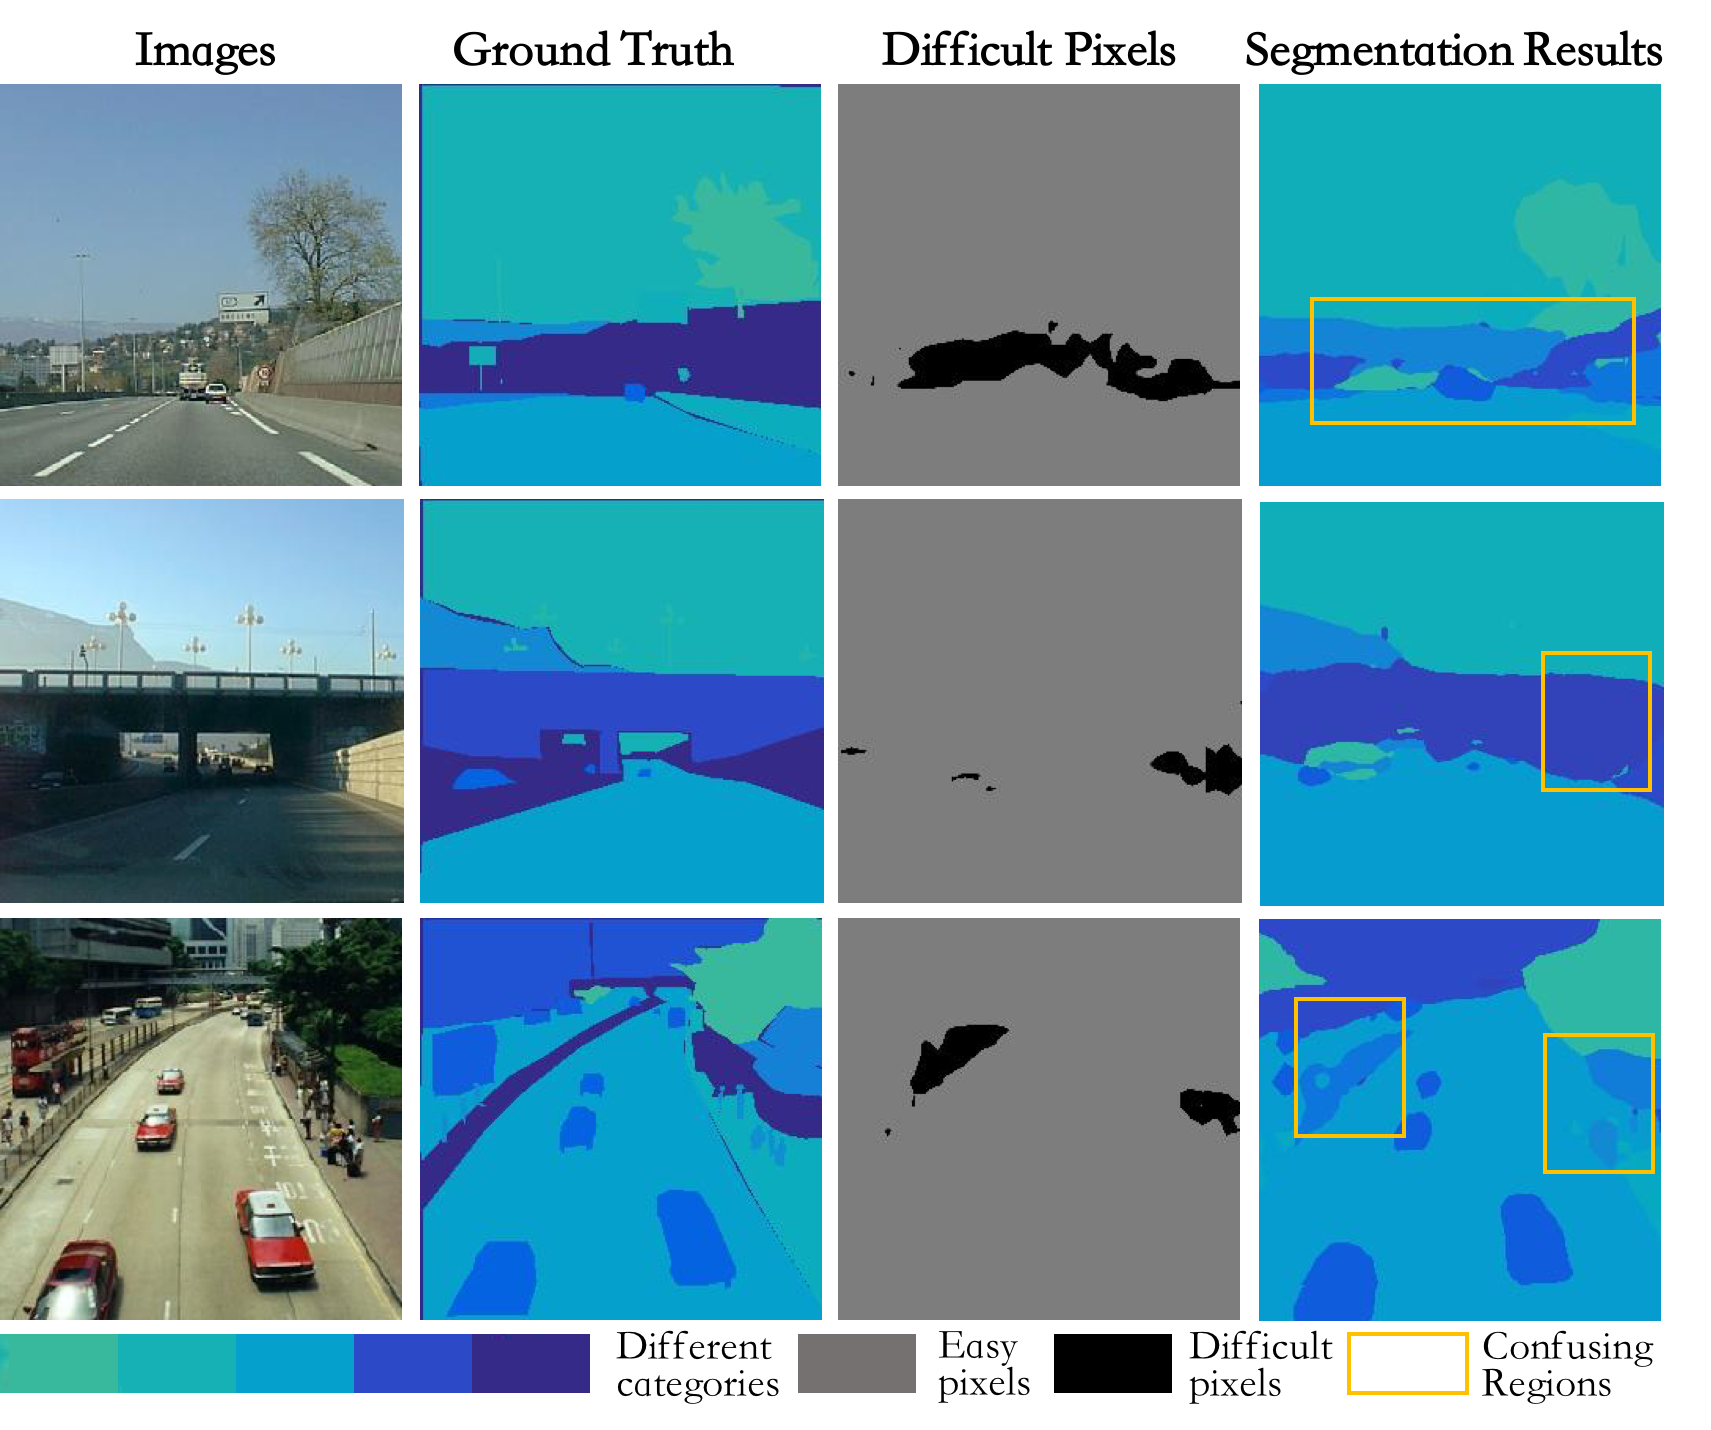
\includegraphics[width=1.9\columnwidth]{fig3.png}
\caption{The visualization predicting result of CCFNet.}
\label{fig:sift}
\end{figure*} 

\section{Experimental results}
\label{s:results}
\noindent
In this section, we will present the detailed information about the implementation of our HMNet. Moreover, we compare our model to the current state-of-the-art methods and achieves superior performances among the existing methods.

\subsection{Network Configuration}
\noindent
The implementation of our HMNet is based on public platform Caffe[30]. The training procedure uses stochastic gradient descent (SGD) algorithm via end-to-end learning. Our model adopt pre-trained models by [29] like most related work on semantic segmentation. The learning rate is initially set to 1e-4 and repeatedly decreased 2 times, corresponding to 3K iterations, 4K iterations, respectively. The momentum and weight decay are set to 0.9 and 0.0001.

Data argumentation is widely applied to semantic segmentation in order to avoid the over-fit. Various kinds of transformations are used to expand the training sizes so as to improve the generalization of the proposed networks. In our experiments, we also employ this kind of methods by expanding the input images 1-2 times and cropping 233*233 randomly for training.  

Larger input size and mini-batch can help improve the segmentation performance. Due to the limitation od both computation and memory, we only use 233*233 images and each mini-batch is 4.


\begin{figure}
\centering
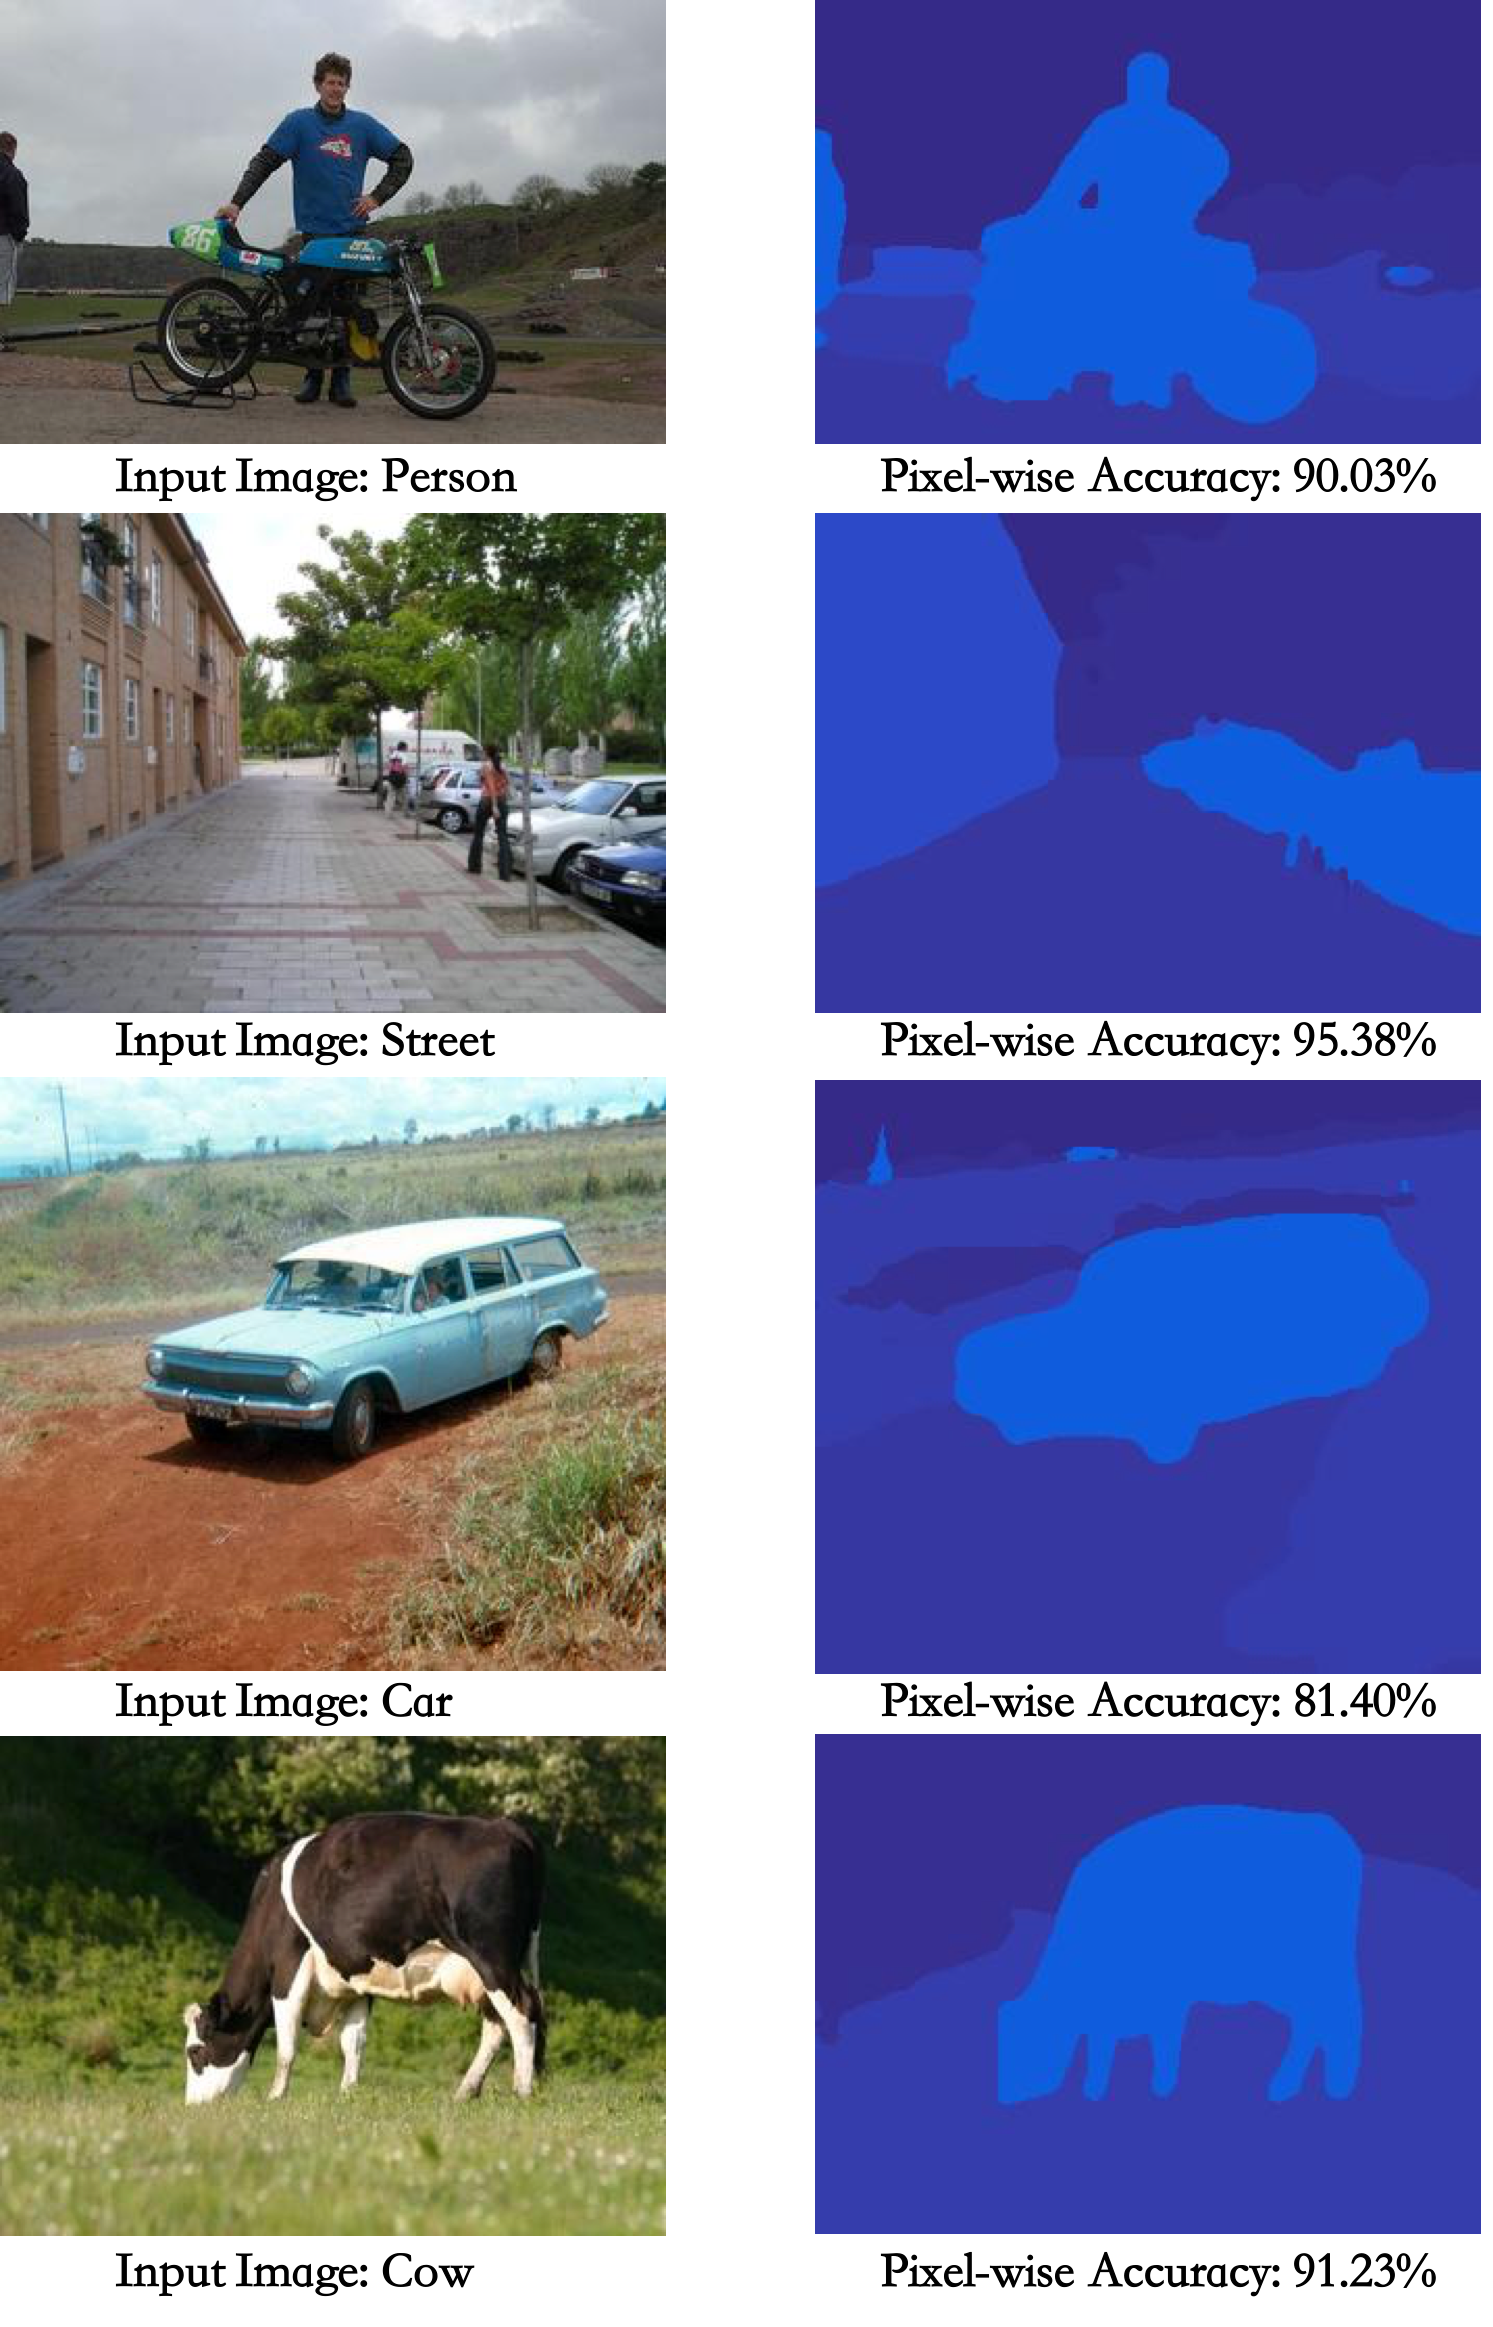
\includegraphics[width=0.95\columnwidth]{fig4.png}
\caption{The predict results on Stanford Background dataset.}
\label{fig:stanford}
\end{figure} 

\subsection{Test}
\noindent
Pixel-level semantic segmentation is usually measured using two accuracy measures: Pixel Accuracy and Class Accuracy. The average pixel accuracy is the percentage of the total number of pixels correctly classified in the test data set, which is usually measured by the intersection-over-union (IoU). The average category accuracy is the average of the correct rate for each category of pixel classification.

\subsection{Datasets}
\noindent
We prove the effectiveness of our HMNet on two semantic segmentation datasets, which are SIFT Flow [11] and Stranford Background [12], respectively. The SIFT Flow dataset contains 2688 samples each has 256x256 pixels with RGB channels. 2488 images are used as a training set while the rest 200 images are used for testing. The dataset defines a total of 33 semantic categories, but the distribution of category is non-uniform.

The Stanford Background dataset contains 715 images with different image sizes, but no more than 320x240 pixels. According to the previous research and testing methods, this paper divides the dataset by 5x cross validation method, and 572 images are used as training samples and 143 samples as the test samples. The Stanford Background dataset contains eight semantic categories, and the category distribution is more balanced than the SIFT Flow dataset

First, we conduct several experiments on SIFT Flow dataset. The results are show in Figure 3 which consist of four columns. The first column presents the input images and second shows the semantic labels. In particular, the third column indicates hard pixels predicted by HMNet while the last column is the segmentation results of the network. As can be seen from the third and fourth columns of Figure 3, the HMNet network can indeed predict the hard pixel samples which are indicated in the yellow square box of Figure 3.

In addition, on the SIFT Flow dataset, we compare the HMNet to other segmentation methods, the experimental results which is shown in Table 1 prove that HMNet achieves an accuracy of 91.6\%, and outperform the current state-of-the-art results.

\subsection{Comparison Results}
\noindent
In order to verify the generalization of the online hard learning of the semantic segmentation, we test the HMNet on another dataset called Stanford Background by using the same architecture and configurations. Table 2 shows that on the Stanford Background dataset, HMNet achieved 89.7\% pixel average accuracy and 75.4\% class average correct rate. Some of the prediction results are shown in Fig. 4, which can be clearly seen Predict the edge information of the results.

\subsection{Results Visualization}
\noindent
This paper presents a semantic segmentation network structure called HMNet. In the semantic prediction of the image, the pixel samples with difficult to identify the images are predicted online. Finally, the secondary identification of these difficult pixels is classified, which improves the correct rate of the whole network segmentation. On the two data sets of SIFT Flow and Stanford Background, HMNet achieved the best segmentation results for two segmented data sets with 91.6\% and 89.7\% test accuracy rates, respectively.


\section{Conclusions}
\noindent

Inspired by the idea of online hard examples mining, we propose a novel cascade coarse to fine segmentation network architecture.
This network include three branches, in which the first is a coarse segmentation network.
While the second branch is an attention network used to predict the difficulty of each pixel.
And the third branch combines the predict results of the first coarse segmentation branch and a fine segmentation network to refine the final segmentation results.
In order to evaluate the segmentation performance of CCFNet, we conduct experiments on two public datasets including Sift Flow Dataset and Stanford Background Dataset. 
We show how to train these three branches in an end-to-end manner. And finally, the experimental results show that compared to all existing models, our CCFNet consistently yields the best performance, with the accuracy of 91.6\% and 89.7\%, respectively.


\vskip 2mm
\zihao{5}
\noindent
\textbf{Acknowledgements}
\vskip 2mm

\zihao{5--}
\noindent
This work was supported in part by the National Science Foundation of China (NSFC) under Grant Nos. 91420106, 90820305, and 60775040, and by the National High-Tech R\&D Program of China under Grant No. 2012AA041402.

\vskip 2mm
\zihao{5}
\noindent
\textbf{\zihao{5}References}
\vskip 2mm


\begin{thebibliography}{99}
\zihao{5-} \addtolength{\itemsep}{-1em}
\vspace {1.5mm}

\bibitem[1]{1}
Krizhevsky A, Sutskever I, Hinton G E. Imagenet classification with deep convolutional neural networks[C]//Advances in neural information processing systems. 2012: 1097-1105.

\bibitem[2]{2}
Simonyan K, Zisserman A. Very deep convolutional networks for large-scale image recognition[J]. arXiv preprint arXiv:1409.1556, 2014.

\bibitem[3]{3}
Szegedy C, Liu W, Jia Y, et al. Going deeper with convolutions[C]//Proceedings of the IEEE Conference on Computer Vision and Pattern Recognition. 2015: 1-9.

\bibitem[4]{4}
Graves A, Mohamed A, Hinton G. Speech recognition with deep recurrent neural networks[C]//Acoustics, speech and signal processing (icassp), 2013 ieee international conference on. IEEE, 2013: 6645-6649.

\bibitem[5]{5}
Sermanet P, Eigen D, Zhang X, et al. Overfeat: Integrated recognition, localization and detection using convolutional networks[J]. arXiv preprint arXiv:1312.6229, 2013.

\bibitem[6]{6}
Ioffe S, Szegedy C. Batch normalization: Accelerating deep network training by reducing internal covariate shift[J]. arXiv preprint arXiv:1502.03167, 2015.

\bibitem[7]{7}
He K, Zhang X, Ren S, et al. Deep residual learning for image recognition[C]//Proceedings of the IEEE Conference on Computer Vision and Pattern Recognition. 2016: 770-778.

\bibitem[8]{8}
Liu C, Yuen J, Torralba A. Sift flow: Dense correspondence across scenes and its applications[J]. IEEE transactions on pattern analysis and machine intelligence, 2011, 33(5): 978-994.

\bibitem[9]{9}
Gould S, Fulton R, Koller D. Decomposing a scene into geometric and semantically consistent regions[C]//Computer Vision, 2009 IEEE 12th International Conference on. IEEE, 2009: 1-8.


\bibitem[10]{10}
Russell C, Kohli P, Torr P H S. Associative hierarchical crfs for object class image segmentation[C]//Computer Vision, 2009 IEEE 12th International Conference on. IEEE, 2009: 739-746.

\bibitem[11]{11}
Kumar M P, Koller D. Efficiently selecting regions for scene understanding[C]//Computer Vision and Pattern Recognition (CVPR), 2010 IEEE Conference on. IEEE, 2010: 3217-3224.

\bibitem[12]{12}
Lempitsky V, Vedaldi A, Zisserman A. Pylon model for semantic segmentation[C]//Advances in neural information processing systems. 2011: 1485-1493.

\bibitem[19]{19}
Farabet C, Couprie C, Najman L, et al. Learning hierarchical features for scene labeling[J]. IEEE transactions on pattern analysis and machine intelligence, 2013, 35(8): 1915-1929.

\bibitem[20]{20}
Couprie C, Farabet C, Najman L, et al. Indoor semantic segmentation using depth information[J]. arXiv preprint arXiv:1301.3572, 2013.

\bibitem[21]{21}
Pinheiro P H O, Collobert R. Recurrent Convolutional Neural Networks for Scene Labeling[C]//ICML. 2014: 82-90.

\bibitem[22]{22}
Shuai B, Wang G, Zuo Z, et al. Integrating parametric and non-parametric models for scene labeling[C]//Proceedings of the IEEE Conference on Computer Vision and Pattern Recognition. 2015: 4249-4258.

\bibitem[23]{23}
Shuai B, Zuo Z, Wang G. Quaddirectional 2d-recurrent neural networks for image labeling[J]. IEEE Signal Processing Letters, 2015, 22(11): 1990-1994.

\bibitem[24]{24}
Shuai B, Zuo Z, Wang B, et al. Dag-recurrent neural networks for scene labeling[C]//Proceedings of the IEEE Conference on Computer Vision and Pattern Recognition. 2016: 3620-3629.

\bibitem[25]{25}
Mostajabi M, Yadollahpour P, Shakhnarovich G. Feedforward semantic segmentation with zoom-out features[C]//Proceedings of the IEEE Conference on Computer Vision and Pattern Recognition. 2015: 3376-3385.

\bibitem[26]{26}
Krizhevsky A, Sutskever I, Hinton G E. Imagenet classification with deep convolutional neural networks[C]//Advances in neural information processing systems. 2012: 1097-1105.

\bibitem[27]{27}
Long J, Shelhamer E, Darrell T. Fully convolutional networks for semantic segmentation[C]//Proceedings of the IEEE Conference on Computer Vision and Pattern Recognition. 2015: 3431-3440.

\bibitem[28]{28}
Chen L C, Papandreou G, Kokkinos I, et al. Semantic image segmentation with deep convolutional nets and fully connected crfs[J]. arXiv preprint arXiv:1412.7062, 2014.

\bibitem[29]{29}
Zhao H, Shi J, Qi X, et al. Pyramid Scene Parsing Network[J]. arXiv preprint arXiv:1612.01105, 2016.

\bibitem[30]{30}
Jia Y, Shelhamer E, Donahue J, et al. Caffe: Convolutional architecture for fast feature embedding[C]//Proceedings of the 22nd ACM international conference on Multimedia. ACM, 2014: 675-678.

\bibitem[31]{31}
Tighe J, Lazebnik S. Superparsing: scalable nonparametric image parsing with superpixels[C]//European conference on computer vision. Springer Berlin Heidelberg, 2010: 352-365.

\bibitem[32]{32}
Tighe J, Lazebnik S. Finding things: Image parsing with regions and per-exemplar detectors[C]//Proceedings of the IEEE conference on computer vision and pattern recognition. 2013: 3001-3008.

\bibitem[33]{33}
Socher R, Lin C C, Manning C, et al. Parsing natural scenes and natural language with recursive neural networks[C]//Proceedings of the 28th international conference on machine learning (ICML-11). 2011: 129-136.

\bibitem[34]{34}
Eigen D, Fergus R. Nonparametric image parsing using adaptive neighbor sets[C]//Computer vision and pattern recognition (CVPR), 2012 IEEE Conference on. IEEE, 2012: 2799-2806.

\bibitem[35]{35}
Singh G, Kosecka J. Nonparametric scene parsing with adaptive feature relevance and semantic context[C]//Proceedings of the IEEE Conference on Computer Vision and Pattern Recognition. 2013: 3151-3157.

\bibitem[36]{36}
Liang M, Hu X. Recurrent convolutional neural network for object recognition[C]//Proceedings of the IEEE Conference on Computer Vision and Pattern Recognition. 2015: 3367-3375.

\begin{strip}
\end{strip}

\begin{biography}[yourphotofilename.eps]
\noindent
\textbf{First A. Author}\ \  Photo. Biographies should be limited to one paragraph consisting of the following: sequentially ordered list of degrees, including years achieved; sequentially ordered places of employ concluding with current employment; associa-tion with any official journals or conferences; major profes-sional and/or academic achievements, i.e., best paper awards, research grants, etc.; any publication information (number of papers and titles of books published); current research interests; association with any professional associations.
\end{biography}

\begin{biography}[yourphotofilename.eps]
\noindent
\textbf{Second B. Author} Photo. Biographies should be limited to one paragraph consisting of the following: sequentially ordered list of degrees, including years achieved; sequentially ordered places of employ concluding with current employment; associa-tion with any official journals or conferences; major profes-sional and/or academic achievements, i.e., best paper awards, research grants, etc.; any publication information (number of papers and titles of books published); current research interests; association with any professional associations.
\end{biography}
\vskip 22mm
\begin{biography}[yourphotofilename.eps]
\noindent
\textbf{Third C. Author}  Photo. Biographies should be limited to one paragraph consisting of the following: sequentially ordered list of degrees, including years achieved; sequentially ordered places of employ concluding with current employment; associa-tion with any official journals or conferences; major profes-sional and/or academic achievements, i.e., best paper awards, research grants, etc.; any publication information (number of papers and titles of books published); current research interests; association with any professional associations.
\end{biography}



  \end{document}


